\documentclass[11pt]{article}
\usepackage[margin=1in]{geometry}
\usepackage{amsmath,booktabs,graphicx,hyperref}
\graphicspath{{../figures/}{figures/}}
\title{Simulating Mechanical Energy Transfer in Rowing\\\large A Simplified One-Dimensional Model}
\author{Gabriel Cirker}
\date{}
\begin{document}\maketitle
\begin{abstract}
This paper uses a simple model to examine how periodic thrust and quadratic drag affect a rowing shell's speed. A prescribed square-wave force accelerates a single mass during the drive and vanishes during recovery. The results illustrate speed fluctuations and energy accounting during a 20-second startup. The calculation does not measure rower efficiency or validate performance against experimental data.
\end{abstract}
\section{Model}
The boat and crew are represented by a single mass $m$ with speed $v$. The equation of motion is
\begin{equation}m\frac{dv}{dt}=F(t)-kv^2.\end{equation}
For the baseline, $m=766.5$ kg, $k=40$ kg/m, and the prescribed thrust is 3000 N for 0.9 seconds in each 2-second cycle, followed by zero thrust. The boat starts from rest. These values are illustrative model inputs, not measurements from a crew.

The model calculates thrust work $W=\int Fv\,dt$, drag work $D=\int kv^3\,dt$ and the change in kinetic energy $\Delta K=m(v_f^2-v_0^2)/2$. In the continuous model $W-D=\Delta K$. Thrust work on the modeled mass is not the rowers' total mechanical or metabolic work. The ratio $\Delta K/W$ describes how much input work remains as kinetic energy at the end of this startup interval; it is not rowing efficiency and depends on the interval chosen.
\section{Method and results}
The equation is integrated with explicit Euler steps of 0.01 seconds for 20 seconds. The baseline average speed over the latter half is 5.785 m/s and the maximum is 6.759 m/s. Thrust work is approximately 141.2 kJ, drag work 132.3 kJ and kinetic energy gain 9.17 kJ. The gain is 6.49\% of thrust work. The difference of about $-316$ J in $W-D-\Delta K$ is a numerical residual from the discrete scheme.

At a 0.005-second step the residual is about $-158$ J; at 0.001 seconds it is about $-31$ J. The corresponding latter-half average speeds are 5.782 and 5.781 m/s. This convergence check addresses discretization, not the physical accuracy of the inputs.
\begin{figure}[ht]\centering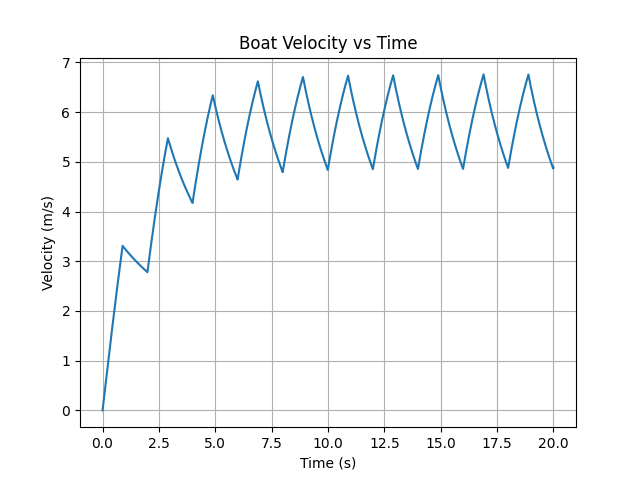
\includegraphics[width=.8\textwidth]{speed_plot.png}\caption{Baseline speed during the 20-second simulation.}\end{figure}
\section{Parameter comparisons and limitations}
With the default step, halving drag raises the latter-half average speed to 8.162 m/s; halving mass gives 5.719 m/s over the same finite interval. Shortening the cycle from 2.0 to 1.5 seconds gives 6.673 m/s, but keeping the drive at 0.9 seconds also increases the drive fraction and input. This is therefore not an isolated comparison at constant work or power.

The model excludes blade slip, rower motion relative to the shell, varying force profiles, wind and waves. It has not been calibrated or compared with measured trajectories. More realistic thrust and drag measurements, timestep checks and experimental validation would be needed before applying the numerical predictions to a crew.

\section{Stroke cycle and energy accounting}
With cycle period $T=2$ s and drive duration $d=0.9$ s, the prescribed force is $F_d$ when $0\leq t\bmod T<d$, and zero otherwise. The resulting duty fraction is $d/T=0.45$. The force acts on the combined modeled mass; it is not a direct measurement of force at an oar handle or a physiological power estimate.

Multiplying the equation of motion by $v$ and integrating gives the continuous energy balance $W-D=\Delta K$. The discrete calculation evaluates force and power at the beginning of each step; the squared velocity update introduces a step-dependent residual. A small residual is a necessary consistency check, but does not verify the drag coefficient or thrust model. Velocity is clipped at zero in the code, so an energy balance would also need to account for that operation if it became active. It is not active in the reported baseline.

\section{Sensitivity profiles}
Figures~\ref{fig:drag}--\ref{fig:stroke} show the complete transient profiles rather than only the summary averages. The mass comparison changes acceleration and stroke-to-stroke fluctuations as well as the finite-interval average. The 20-second averages do not prove that a periodic steady state has been reached. Lower drag changes the relationship between thrust, speed and work, so it is not a comparison at equal mechanical power. The higher-rate case uses a longer fraction of each cycle for the drive and therefore changes more than stroke frequency.
\begin{figure}[ht]\centering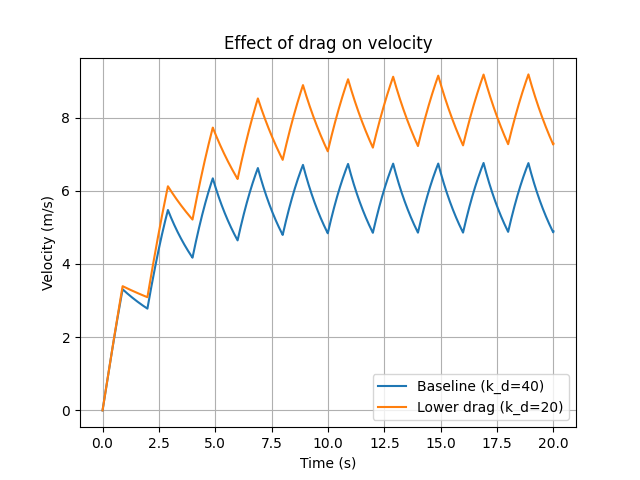
\includegraphics[width=.75\textwidth]{drag_effect.png}\caption{Velocity for baseline and lower drag.}\label{fig:drag}\end{figure}
\begin{figure}[ht]\centering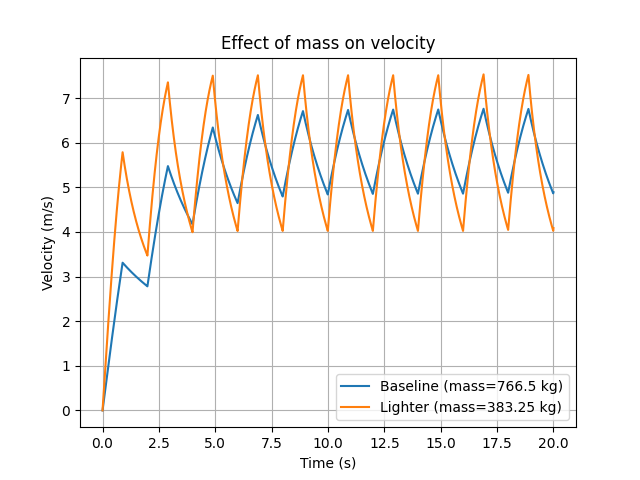
\includegraphics[width=.75\textwidth]{mass_effect.png}\caption{Velocity for baseline and lower mass.}\label{fig:mass}\end{figure}
\begin{figure}[ht]\centering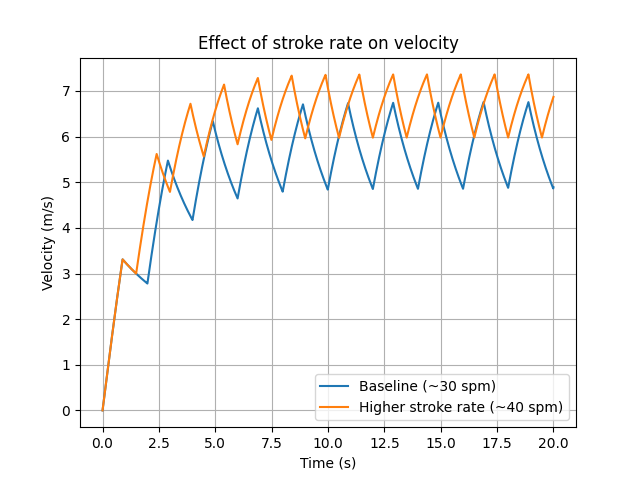
\includegraphics[width=.75\textwidth]{stroke_effect.png}\caption{Velocity for two cycle periods with fixed drive duration.}\label{fig:stroke}\end{figure}
\begin{figure}[ht]\centering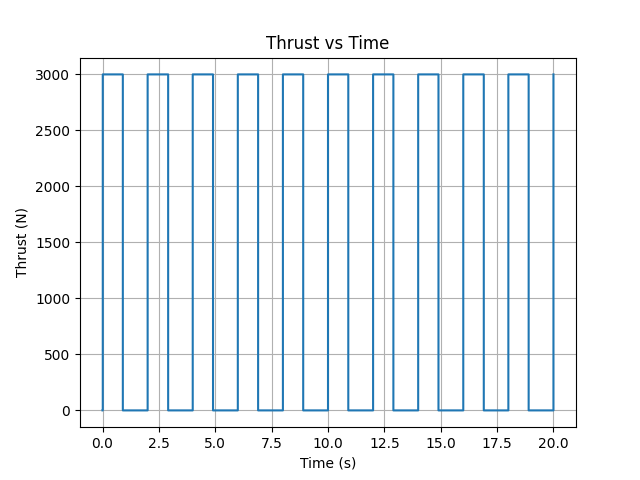
\includegraphics[width=.75\textwidth]{thrust_plot.png}\caption{Prescribed thrust profile.}\end{figure}

\section{Context and further work}
Rowing involves moving body segments, oar-water interactions and hull motion that cannot be resolved by this single-mass model. A biomechanical review by Baudouin and Hawkins discusses performance factors and velocity fluctuations \cite{baudouin}; it provides context rather than validation of the present parameter choices. A useful next step is to fit time-resolved thrust and speed to independent measurements, assess parameter uncertainty, and compare predictions with held-out strokes. A longer simulation with a cycle-to-cycle convergence criterion would distinguish startup behavior from periodic operation. Comparisons of stroke rates should specify whether mean thrust, work per stroke, or average power is held fixed.
\section{Moving-mass extension}
The lumped model makes the hull and crew move as one mass. To examine recovery motion, I consider a reduced model in which the crew center of mass moves relative to the hull. Let $m_b$ be the hull-fixed mass, $m_r$ the moving mass, $M=m_b+m_r$, $X_b$ the hull position, and $x_r$ the crew position relative to the hull. The combined center of mass is
\begin{equation}X_c=X_b+\frac{m_r}{M}x_r.\end{equation}
If external surge forces are represented by thrust $F$ and drag $D$, differentiating twice gives
\begin{equation}M\ddot X_b=F-D-m_r\ddot x_r.\end{equation}
A prescribed internal acceleration changes hull acceleration even though it does not change total momentum in an isolated system. The sign depends on the coordinate direction. The relation follows from the two-mass assumptions; it does not determine crew trajectory, blade force, or internal work. Measured or explicitly prescribed motion would be needed to evaluate the term. The appendix's prescribed trajectory uses a half-cosine drive followed by a cosine, fifth-order polynomial, or blended recovery. I reconstructed this component as \texttt{src/slide\_kinematics.py}; tests compare its analytic derivatives with finite differences away from transitions. Position and velocity are continuous at the drive--recovery boundary, but acceleration may jump there. This component alone does not reproduce the original multibody or IMU figures.

\section{Pitch and disturbance resistance: a proposed surrogate}
A possible extension represents pitch $\theta$ with effective inertia, damping, and restoring stiffness:
\begin{equation}I_\theta\ddot\theta+c_\theta\dot\theta+k_\theta\theta=\tau(t).\end{equation}
A phenomenological drag law can then be written $D=kv^2(1+\alpha\theta^2+\beta\dot\theta^2)$ for forward motion. The coefficients must carry units consistent with the dimensionless multiplier and must be fitted or independently supported. The incremental work $\int kv^3(\alpha\theta^2+\beta\dot\theta^2)dt$ compares terms at the same instantaneous speed. It is not automatically the difference between two coupled simulations, because changing drag can also change speed and pitch. These moving-mass, pitch, and resistance equations are proposed extensions; the included scripts implement the baseline surge model only. I do not treat the illustrative synthetic results in the longer manuscript as reproduced or experimentally validated here.

\section{Speed fluctuations and power}
For $v=\bar v+u$, with $\langle u\rangle=0$, the exact identity is
\begin{equation}\langle v^3\rangle=\bar v^3+3\bar v\langle u^2\rangle+\langle u^3\rangle.\end{equation}
For nonnegative speeds, convexity implies $\langle v^3\rangle\geq\bar v^3$. Under this model a variable speed at fixed mean speed and fixed drag coefficient requires at least as much average drag power as constant speed. This comparison does not establish that reducing hull speed fluctuations always improves race performance: changing technique may alter propulsion, crew motion, and other losses. The model makes the energetic assumption explicit rather than providing a coaching prescription.

\section{Measurement and system identification}
To connect the model to measurements, a future protocol could synchronize a hull-mounted inertial measurement unit, independent speed measurements, stroke events, and a force or power proxy. Sensor orientation, gravity removal, mounting, calibration, sampling and filtering should be documented before calculating acceleration or pitch features. Integrating acceleration to obtain speed requires independent drift correction. A rowing sensor review discusses measurement choices and their constraints \cite{worsey}. Events detected from a hull signal should be checked against an independent stroke reference rather than assumed to coincide with the catch or finish.

Let $y_i$ denote measured waveforms or features and $\hat y_i(\psi)$ their model counterparts. A candidate fit minimizes $\sum_i (y_i-\hat y_i)^T\Sigma_i^{-1}(y_i-\hat y_i)+\lambda\Omega(\psi)$ over physically admissible parameters. The covariance or weighting matrix $\Sigma_i$ and regularizer $\Omega$ must be specified before fitting. Sensitivity rank, profile likelihood or comparable diagnostics are needed to examine whether parameters can be separated; a good waveform fit alone does not prove identifiability. Validation should use held-out sessions or trials, report uncertainty and compare predictions with independently measured outcomes. The source manuscript's synthetic demonstration is distinct from such empirical validation; its advanced scripts and input data were not available as runnable files in this project.

\begin{thebibliography}{9}
\bibitem{baudouin} A. Baudouin and D. Hawkins, ``A biomechanical review of factors affecting rowing performance,'' \emph{British Journal of Sports Medicine}, 36, 396--402, 2002. \url{https://bionics.seas.ucla.edu/education/Rowing/Math_Model_2002_01.pdf}.
\bibitem{worsey} M. T. O. Worsey, H. G. Espinosa, J. B. Shepherd and D. V. Thiel, ``A Systematic Review of Performance Analysis in Rowing Using Inertial Sensors,'' \emph{Electronics}, 8(11), 1304, 2019. \url{https://doi.org/10.3390/electronics8111304}.
\end{thebibliography}

\end{document}
